\documentclass[tikz, usenames, dvipsnames]{standalone}
\usepackage{pgfplots}
\usepgfplotslibrary{groupplots}
\pgfplotsset{height=7.5cm, width=14.5cm, compat=1.18}
\usepackage{tikz}
\usepackage{gensymb}
\usepackage{amsmath}

\begin{document}
	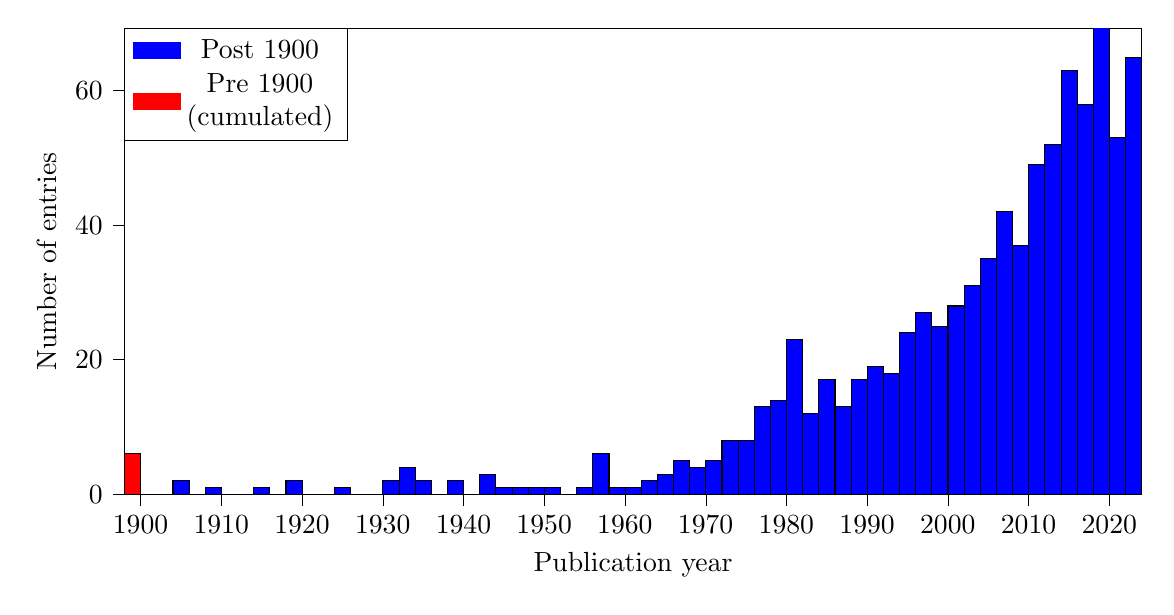
\begin{tikzpicture}
		%\draw[draw=black] (-1.3,-1.2) rectangle ++(14.5cm,7cm);
		
		\begin{axis}[
			tick align=outside,
			tick pos=left,
			xlabel={Publication year},
			xmin=1898, xmax=2024,
			xtick style={color=black},
			ylabel={Number of entries},
			ymin=0, ymax=69.3,
			ytick style={color=black},
			legend style={},
			legend style={anchor=north west, at={(0,1)}, xshift=-0.2pt, yshift=+0.2pt, align=center},
			/pgf/number format/.cd,
			1000 sep={},
			]
			
			\addplot[draw=blue, fill=blue, area legend] (1,1);
			\addplot[draw=red, fill=red, area legend] (1,1);
			
			\addlegendentry{Post 1900}
			\addlegendentry{Pre 1900\\(cumulated)}
			
			\draw[draw=black,fill=red] (axis cs:1894,0) rectangle (axis cs:1896,0);
			\draw[draw=black,fill=red] (axis cs:1896,0) rectangle (axis cs:1898,0);
			\draw[draw=black,fill=red] (axis cs:1898,0) rectangle (axis cs:1900,6);
			\draw[draw=black,fill=blue] (axis cs:1900,0) rectangle (axis cs:1902,0);
			\draw[draw=black,fill=blue] (axis cs:1902,0) rectangle (axis cs:1904,0);
			\draw[draw=black,fill=blue] (axis cs:1904,0) rectangle (axis cs:1906,2);
			\draw[draw=black,fill=blue] (axis cs:1906,0) rectangle (axis cs:1908,0);
			\draw[draw=black,fill=blue] (axis cs:1908,0) rectangle (axis cs:1910,1);
			\draw[draw=black,fill=blue] (axis cs:1910,0) rectangle (axis cs:1912,0);
			\draw[draw=black,fill=blue] (axis cs:1912,0) rectangle (axis cs:1914,0);
			\draw[draw=black,fill=blue] (axis cs:1914,0) rectangle (axis cs:1916,1);
			\draw[draw=black,fill=blue] (axis cs:1916,0) rectangle (axis cs:1918,0);
			\draw[draw=black,fill=blue] (axis cs:1918,0) rectangle (axis cs:1920,2);
			\draw[draw=black,fill=blue] (axis cs:1920,0) rectangle (axis cs:1922,0);
			\draw[draw=black,fill=blue] (axis cs:1922,0) rectangle (axis cs:1924,0);
			\draw[draw=black,fill=blue] (axis cs:1924,0) rectangle (axis cs:1926,1);
			\draw[draw=black,fill=blue] (axis cs:1926,0) rectangle (axis cs:1928,0);
			\draw[draw=black,fill=blue] (axis cs:1928,0) rectangle (axis cs:1930,0);
			\draw[draw=black,fill=blue] (axis cs:1930,0) rectangle (axis cs:1932,2);
			\draw[draw=black,fill=blue] (axis cs:1932,0) rectangle (axis cs:1934,4);
			\draw[draw=black,fill=blue] (axis cs:1934,0) rectangle (axis cs:1936,2);
			\draw[draw=black,fill=blue] (axis cs:1936,0) rectangle (axis cs:1938,0);
			\draw[draw=black,fill=blue] (axis cs:1938,0) rectangle (axis cs:1940,2);
			\draw[draw=black,fill=blue] (axis cs:1940,0) rectangle (axis cs:1942,0);
			\draw[draw=black,fill=blue] (axis cs:1942,0) rectangle (axis cs:1944,3);
			\draw[draw=black,fill=blue] (axis cs:1944,0) rectangle (axis cs:1946,1);
			\draw[draw=black,fill=blue] (axis cs:1946,0) rectangle (axis cs:1948,1);
			\draw[draw=black,fill=blue] (axis cs:1948,0) rectangle (axis cs:1950,1);
			\draw[draw=black,fill=blue] (axis cs:1950,0) rectangle (axis cs:1952,1);
			\draw[draw=black,fill=blue] (axis cs:1952,0) rectangle (axis cs:1954,0);
			\draw[draw=black,fill=blue] (axis cs:1954,0) rectangle (axis cs:1956,1);
			\draw[draw=black,fill=blue] (axis cs:1956,0) rectangle (axis cs:1958,6);
			\draw[draw=black,fill=blue] (axis cs:1958,0) rectangle (axis cs:1960,1);
			\draw[draw=black,fill=blue] (axis cs:1960,0) rectangle (axis cs:1962,1);
			\draw[draw=black,fill=blue] (axis cs:1962,0) rectangle (axis cs:1964,2);
			\draw[draw=black,fill=blue] (axis cs:1964,0) rectangle (axis cs:1966,3);
			\draw[draw=black,fill=blue] (axis cs:1966,0) rectangle (axis cs:1968,5);
			\draw[draw=black,fill=blue] (axis cs:1968,0) rectangle (axis cs:1970,4);
			\draw[draw=black,fill=blue] (axis cs:1970,0) rectangle (axis cs:1972,5);
			\draw[draw=black,fill=blue] (axis cs:1972,0) rectangle (axis cs:1974,8);
			\draw[draw=black,fill=blue] (axis cs:1974,0) rectangle (axis cs:1976,8);
			\draw[draw=black,fill=blue] (axis cs:1976,0) rectangle (axis cs:1978,13);
			\draw[draw=black,fill=blue] (axis cs:1978,0) rectangle (axis cs:1980,14);
			\draw[draw=black,fill=blue] (axis cs:1980,0) rectangle (axis cs:1982,23);
			\draw[draw=black,fill=blue] (axis cs:1982,0) rectangle (axis cs:1984,12);
			\draw[draw=black,fill=blue] (axis cs:1984,0) rectangle (axis cs:1986,17);
			\draw[draw=black,fill=blue] (axis cs:1986,0) rectangle (axis cs:1988,13);
			\draw[draw=black,fill=blue] (axis cs:1988,0) rectangle (axis cs:1990,17);
			\draw[draw=black,fill=blue] (axis cs:1990,0) rectangle (axis cs:1992,19);
			\draw[draw=black,fill=blue] (axis cs:1992,0) rectangle (axis cs:1994,18);
			\draw[draw=black,fill=blue] (axis cs:1994,0) rectangle (axis cs:1996,24);
			\draw[draw=black,fill=blue] (axis cs:1996,0) rectangle (axis cs:1998,27);
			\draw[draw=black,fill=blue] (axis cs:1998,0) rectangle (axis cs:2000,25);
			\draw[draw=black,fill=blue] (axis cs:2000,0) rectangle (axis cs:2002,28);
			\draw[draw=black,fill=blue] (axis cs:2002,0) rectangle (axis cs:2004,31);
			\draw[draw=black,fill=blue] (axis cs:2004,0) rectangle (axis cs:2006,35);
			\draw[draw=black,fill=blue] (axis cs:2006,0) rectangle (axis cs:2008,42);
			\draw[draw=black,fill=blue] (axis cs:2008,0) rectangle (axis cs:2010,37);
			\draw[draw=black,fill=blue] (axis cs:2010,0) rectangle (axis cs:2012,49);
			\draw[draw=black,fill=blue] (axis cs:2012,0) rectangle (axis cs:2014,52);
			\draw[draw=black,fill=blue] (axis cs:2014,0) rectangle (axis cs:2016,63);
			\draw[draw=black,fill=blue] (axis cs:2016,0) rectangle (axis cs:2018,58);
			\draw[draw=black,fill=blue] (axis cs:2018,0) rectangle (axis cs:2020,70);
			\draw[draw=black,fill=blue] (axis cs:2020,0) rectangle (axis cs:2022,53);
			\draw[draw=black,fill=blue] (axis cs:2022,0) rectangle (axis cs:2024,65);
		\end{axis}
		
	\end{tikzpicture}
	
\end{document}